\documentclass[11pt]{article}
\usepackage[english]{babel}
\usepackage[utf8]{inputenc}
\usepackage{fancyhdr}
\usepackage{graphicx}

\def\Name{Ran Liao}
\def\Topic{Interaction Diagram}

\title{\textbf{\Topic}}
\author{\Name}
\markboth{Notes on \Topic\ }{Notes on \Topic\ }
\date{\today}
 
\pagestyle{fancy}
\fancyhf{}
\rhead{\date{\today} }
\lhead{Notes on \Topic\ }
\rfoot{\thepage}

\textheight=9in
%\textwidth=6.5in
\topmargin=-.75in
%\oddsidemargin=0in
%\evensidemargin=0in
 
\begin{document}
\maketitle
\noindent\makebox[\linewidth]{\rule[8pt]{5in}{0.5pt}}



\section*{Overview}

An interaction diagram shows how objects interact as messages are passed between them. UML supports two types of interaction diagrams.

\begin{itemize}
	\item \textbf{Sequence Diagram}
	\item \textbf{Collaboration Diagram}
\end{itemize}

\section*{Sequence Diagram}

Use a sequence diagram when the transfer of information is the focus of attention.

\begin{figure}[h]
	\centering
	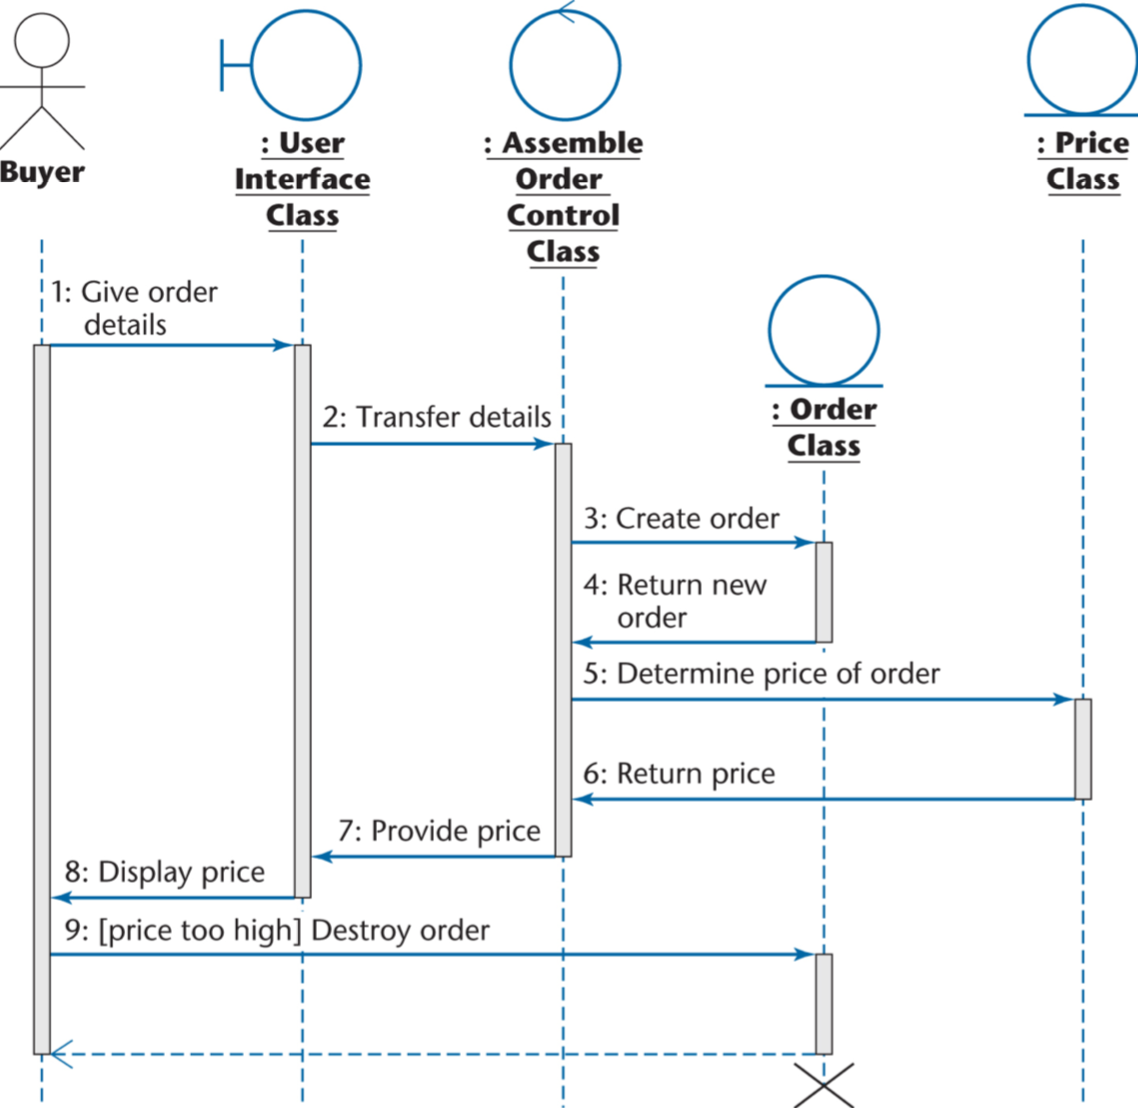
\includegraphics[width=0.7\linewidth]{images/SequenceDiagram.png}
	\caption{Sequence Diagram}
	\label{fig:SequenceDiagram}
\end{figure}

\section*{Collaboration Diagram}

Use a collaboration diagram when concentrating on the classes.

\begin{figure}[h]
	\centering
	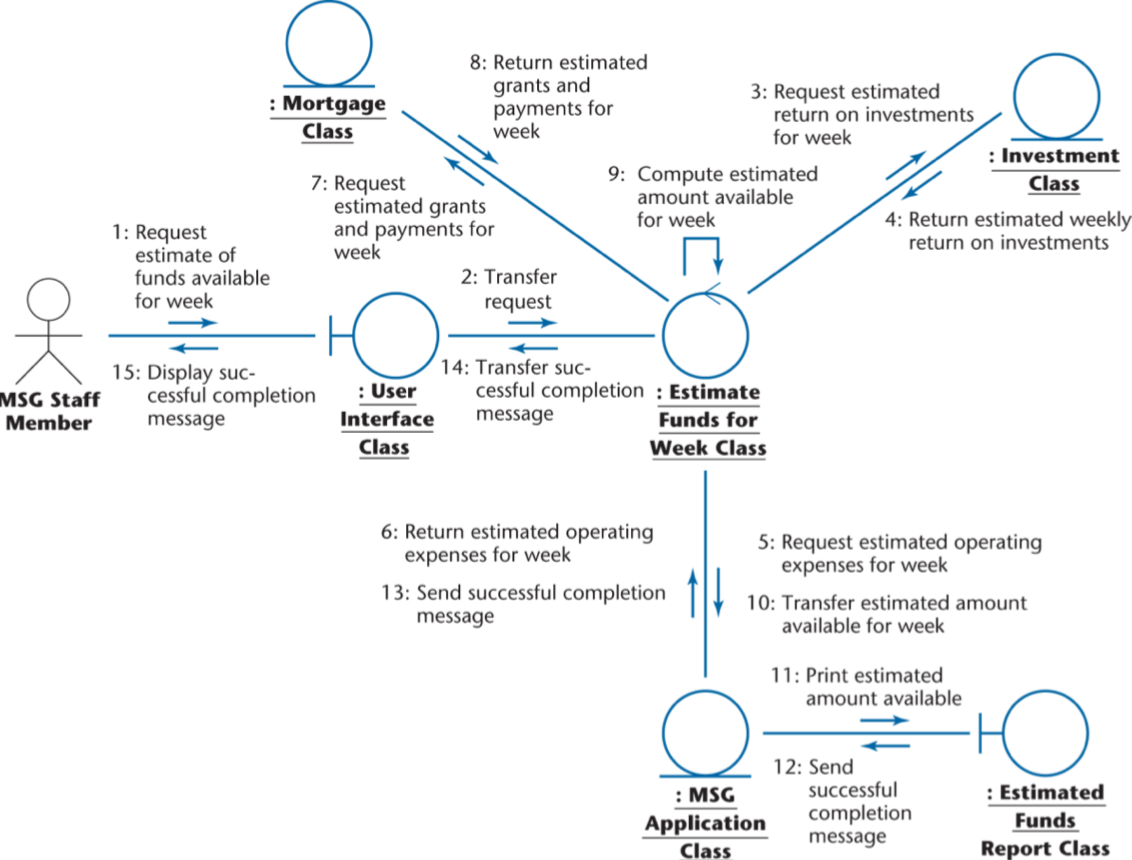
\includegraphics[width=0.7\linewidth]{images/CollaborationDiagram.png}
	\caption{Collaboration Diagram}
	\label{fig:CollaborationDiagram}
\end{figure}



\end{document}